%%%
%%% CARREGANDO PACOTES
%%%

\documentclass[
	openright, % Capítulos começam em página direita
	twoside,   % Impressão frente e verso
	a4paper,   % Tamanho do papel
	english,   % Idioma adiciona para hifenizaçãoo
	brazil     % O ultimo é o idioma principal
]{abntex2}

\usepackage{lmodern}                               % Usa família de fontes Latin Modern
\renewcommand*\familydefault{\sfdefault}           % Usa fonte Latin Modern Sans (Sem serifa)
\usepackage[T1]{fontenc}                           % Codifição Type1 para a fonte (Fontes de 8 bits para incluir as fontes do alfabeto brasileiro)
\usepackage[UTF8]{inputenc}                        % Codificação unicode "UTF8"
\usepackage{microtype}                             % Melhorias na justificação (Evita bad/underfullbox)
\usepackage{indentfirst}                           % Indenta o primeiro parágrafo da seção
%\usepackage{lastpage}                              % Conta o número total de páginas (P/ Ficha catalográfica)

\usepackage{multirow}                              % Suporte a células de tabelas com multilinhas
\usepackage{amssymb}                               % Símbolos matemáticos
\usepackage{enumitem}                              % Melhoria no suporte aos ambientes de numeração

\usepackage{color}                                 % Suporte a cores
\definecolor{blue}{RGB}{41,5,195}                  % Alterando o aspécto da cor Azul
\usepackage{graphicx}                              % Suporte a gráficos e figuras

\usepackage[alf]{abntex2cite}                      % Citações no padrão ABNT



%%%
%%% NOVOS COMANDOS
%%%

\renewcommand{\imprimircapa}{
	\begin{capa}%
		\center
		\begin{minipage}{1.0\textwidth}
			\begin{minipage}[c]{0.14\textwidth}
				\centering
				
\includegraphics[width=0.8\textwidth]{figuras/brasao_ufba.jpg}
			\end{minipage}
			\hfill
			\begin{minipage}[c]{0.7\textwidth}
				\centering
				\ABNTEXchapterfont\large\textbf{\MakeUppercase\imprimirinstituicao}
			\end{minipage}
			\hfill
			\begin{minipage}[c]{0.14\textwidth}
				
\includegraphics[width=0.9\textwidth]{figuras/brasao_poli.jpg}
			\end{minipage}
		\end{minipage}
		\\
		\vspace*{2cm}
		{\ABNTEXchapterfont\large\MakeUppercase\imprimirautor}
		\vfill
		{\ABNTEXchapterfont\bfseries\LARGE\MakeUppercase\imprimirtitulo}
		\vfill
		{\large\MakeUppercase\imprimirlocal} \\
		{\large\MakeUppercase\imprimirdata}
		\vspace*{1cm}
	\end{capa}
}

\renewcommand{\imprimirfolhaderosto}{
	\begin{folhaderosto}%
		\centering
		{\ABNTEXchapterfont\large\textbf{\MakeUppercase\imprimirinstituicao}}\\
		\vspace*{2cm}
		{\ABNTEXchapterfont\large\MakeUppercase\imprimirautor}\\
		\vfill
		{\ABNTEXchapterfont\bfseries\LARGE\MakeUppercase\imprimirtitulo}
		\vspace*{0.5cm}
		\begin{center}
			\hspace{.35\textwidth}
			\begin{minipage}{.5\textwidth}
				\large\imprimirpreambulo
				\vspace*{0.5cm}
			\end{minipage}%
		\end{center}
		{\large Orientador: Prof. Dr. \imprimirorientador\\
		\vspace*{\fill}}
		{\large\MakeUppercase\imprimirlocal} \\
		{\large\MakeUppercase\imprimirdata}
		\vspace*{1cm}
	\end{folhaderosto}
}

\newcommand{\imprimirfolhadeaprovacao}[2]{
	\begin{folhadeaprovacao}%
		\centering
		{\ABNTEXchapterfont\large\textbf{\MakeUppercase{Termo de Aprovação}}}\\
		\vspace*{0.5cm}
		{\ABNTEXchapterfont\large\MakeUppercase\imprimirautor}\\
		\vspace*{4cm}
		{\ABNTEXchapterfont\bfseries\LARGE\MakeUppercase\imprimirtitulo}
		\vspace*{0.5cm}
		\begin{center}
			\hspace{.35\textwidth}
			\begin{minipage}{.5\textwidth}
				\large
				Este Trabalho de Graduação foi julgado adequado para a obtenção do grau de Engenheiro Eletricista e aprovado em sua forma final pela Comissão Examinadora e pelo Colegiado do Curso de Graduação em Engenharia Elétrica da Universidade Federal da Bahia.
				\vspace*{0.5cm}
			\end{minipage}%
		\end{center}
		\vfill
		\assinatura{Prof. Dr. \imprimirorientador \\Orientador\\}
		\assinatura{#1 \\ Examinador\\}
		\assinatura{#2 \\ Examinador}
		\vspace*{2cm}
		{\large\MakeUppercase\imprimirlocal} \\
		{\large\MakeUppercase\imprimirdata}
		\vspace*{1cm}
	\end{folhadeaprovacao}
}

\newcommand{\imprimirdedicatoria}[1]{
	\begin{dedicatoria}
		\vspace*{\fill}
		\centering
		\noindent
		\textit{#1}
		\vspace*{\fill}
	\end{dedicatoria}
}

\newcommand{\imprimirepigrafe}[2]{
	\begin{epigrafe}
		\vspace*{\fill}
		\begin{flushright}
			\textit{``#1''\\
				(#2)}
		\end{flushright}
	\end{epigrafe}
}

%%%
%%% Dados do trabalho
%%%

\instituicao{Universidade Federal da Bahia\par
	Escola Politécnica\par
	Curso de Graduação em Engenharia Elétrica
}

\tipotrabalho{Trabalho Final de Graduação}

\preambulo{Trabalho apresentado ao Curso de Graduação em Engenharia Elétrica da Universidade Federal da Bahia como parte dos requisitos para a obtenção do título de Engenheiro Eletricista.}


% informações do PDF
\makeatletter
\hypersetup{
	%pagebackref=true,
	pdftitle={\@title}, 
	pdfauthor={\@author},
	pdfsubject={\imprimirpreambulo},
	pdfcreator={LaTeX with abnTeX2},
	pdfkeywords={abnt}{latex}{abntex}{abntex2}{trabalho acadêmico}, 
	colorlinks=true,       		% false: boxed links; true: colored links
	linkcolor=black,          	% color of internal links
	citecolor=black,        		% color of links to bibliography
	filecolor=black,      		% color of file links
	urlcolor=black,
	bookmarksdepth=4
}
\makeatother

% O tamanho do parágrafo é dado por:
\setlength{\parindent}{1.3cm}

% Controle do espaçamento entre um parágrafo e outro:
\setlength{\parskip}{0.2cm}  % tente também \onelineskip


\titulo{Uso do Beaglebone Black como um sistema de aquisição de dados}

\autor{Lucas Lima Rodrigues}

\local{Salvador}

\data{2016}

\orientador{Antônio Cezar de Castro Lima}

\makeindex

\AtBeginDocument{
	\frenchspacing 
	\pretextual
	
	\imprimircapa
	\imprimirfolhaderosto
	
	\imprimirfolhadeaprovacao{Prof. Dra. Ana Isabela Araújo Cunha}{Prof. Me. Leroy Umasi Ramos}
	
	\imprimirdedicatoria{
		Este trabalho é dedicado e minha família, minha vó minha tia e todos os amigos e professores que acreditaram em mim.
	}
	
	\imprimirepigrafe{O único lugar aonde o sucesso vem antes do trabalho é no dicionário.}{Albert Einstein}
	
	\begin{agradecimentos}
	
	Aos meus pais e meu irmão, aos meus tios, João e Simone, e à Aline, minha ``prima-irmã'' e afilhada. Enfim, a toda minha primeira e grande família: ensinamentos e valores que transcendem em muito a importância de títulos acadêmicos.
	
	À minha segunda família: mãe Zélia, irmãos Rodrigo, Juliana, Bruno, Iara, Ariel, Karen e tantos outros, que foram se agregando, compartilhando e tornando a jornada mais fácil. Ao engrandecimento que me trouxeram.
	
	À Petúnia, pelo amor, incentivo e uma carinhosa paciência, difíceis de traduzir em palavras. Também aos seus pais, Wilson e Derci, pelo acolhimento e exemplo.
	
	Aos amigos da UFBA, melhor legado que levo desse curso: Simon, Jivago, Adinaílson, Ana Rita, Túlio, Fred, Roberto e Tássio. Poderia discorrer muito sobre a contribuição que cada um deu nestes longos anos de graduação, mas a beleza está na cumplicidade da amizade.
	
	Aos professores - concordando ou não com suas metodologias, todo aprendizado adquirido foi válido.
	
	Aos orientadores Edson e Ana Isabela, meu mais profundo apreço pelo auxílio, desde 2011, na iniciação científica, até agora, no presente trabalho.
	
\end{agradecimentos}
	
	\setlength{\absparsep}{18pt} % ajusta o espaçamento dos parágrafos do resumo
\begin{resumo}
	Este é o resumo em Português
	
	\textbf{Palavras-chaves}: sistema de aquisição de dados, linux embarcado, beaglebone black, interface USB.
\end{resumo}

% resumo em inglês
\begin{resumo}[Abstract]
	\begin{otherlanguage*}{english}
		English abstract
		\vspace{\onelineskip}
		
		\noindent 
		\textbf{Key-words}: data acquisition systems, embedded linux, beaglebone black, USB interface.
	\end{otherlanguage*}
\end{resumo}
	
	%Sumário
	\tableofcontents*
	\cleardoublepage
	
	%lista de figuras
	\pdfbookmark[0]{\listfigurename}{lof}
	\listoffigures*
	\cleardoublepage
	
	%lista de tabelas
	\pdfbookmark[0]{\listtablename}{lot}
	\listoftables*
	\cleardoublepage
	
	%Lista de siglas
	\begin{siglas}
	\item[ADC] \emph{Analog-to-Digital Converter}
	\item[ARM] \emph{Advanced RISC Machine}
	\item[CNC]  \emph{Computer Numeric Control} (Máquina de usinagem de peças metálicas)
	\item[CPU] \emph{Central Processing Unit}
	\item[BBB] \emph{Beaglebone Black}
	\item[DAQ] \emph{Data Acquisition Systems}
	\item[DC] Tensão Continua (\emph{Direct Current})
	\item[DDR] \emph{Double Data Rate} (Tecnologia de memoria RAM)
	\item[DSI] \emph{Display Serial Interface}
	\item[DSL] \emph{Digital Subscriber Line}
	\item[DOS] \emph{Disk Operating System}
	\item[E-Linux] \emph{Embedded Linux}
	\item[IP] \emph{Internet Protocol}
	\item[ISO] \emph{International Organization for Standardization}
	\item[Freq.] Frequência
	\item[FAT] \emph{File Allocation Table} (Sistema de arquivo criado pela Microsoft para gerenciar acesso de arquivos em partições de disco)
	\item[GUI] \emph{Graphical User Interface}
	\item[GPU] \emph{Graphics Processing Unit}
	\item[GTK+] \emph{Framework} multiplataforma para criação de programas com interface gráfica 
	\item[HDMI] \emph{High-Definition Multimedia Interface}
	\item[I2C] \emph{Inter-Integrated Circuit} 
	\item[I/O] \emph{Input \& Output pin}
	\item[JTAG] \emph{Joint Test Action Group} (Conector utilizado para teste de circuitos eletrônicos).
	\item[LAN] \emph{Local Area Network}
	\item[LCD] \emph{Liquid Crystal Display} 
	\item[LDO] \emph{Low-dropout regulator} (Regulador de tensão capaz de regular a voltagem de saída quando a tensão de estrada está próxima da tensão de saída)
	\item[MIPS] \emph{Microprocessor without Interlocked Pipeline Stage}
	\item[NI] \emph{National Instruments}
	\item[OSI] \emph{Open Systems Interconnection}
	\item[PC] \emph{Personal Computer}
	\item[PCI] Padrão de barramento interno para computadores
	\item[PCI-E] PCI \emph{Express}
	\item[PDA] \emph{Personal Digital Assistant}
	\item[PRU] Programmable Real-Time Unit
	\item[PWM] Pulse Width Modulation
	\item[Qt] Outra \emph{framework} multiplataforma para criação de programas com interface gráfica
	\item[RAM] \emph{Random Access Memory}
	\item[RCA] Conector criado pela \emph{Radio Corporation of America}
	\item[rev.] \emph{revision}
	\item[RJ45] Conector utilizado no padrão Ethernet
	\item[RS232] Padrão de comunicação serial
	\item[RS485] Outro padrão de comunicação serial
	\item[SO] Sistema operacional
	\item[SOC] \emph{System-on-chip}
	\item[SPI] \emph{Serial Peripheral Interface}
	\item[SSH] \emph{Secure Shell}
	\item[UART] \emph{Universal Asynchronous Receiver/Transmitter}
	\item[USB] \emph{Universal Serial Bus}
	\item[Wi-Fi] Padrão de comunicação sem fio IEEE 802.11
\end{siglas}
	\cleardoublepage
	
	\textual
	\pagenumbering{arabic}
	\setcounter{page}{1}
}


\begin{document}
	\chapter{Introdução}
	\label{ch:introduction}
	Um sistema de aquisição de dados, ou DAQ do inglês \emph{Data Acquisition Systems}, é um dispositivo, ou um conjunto deles, capaz de coletar, armazenar e distribuir uma determinada informação de tal forma que esta, posteriormente, possa ser manipulada ou utilizada para entender melhor o fenômeno. Na prática esses sistemas são utilizados para capturar dados de uma determinada variável física de um processo, geralmente vinda de um sensor.

Inicialmente os sistemas de aquisição de dados eram dispositivos eletromecânicos que mostravam uma determinada grandeza física em um visor analógico e registravam as mesmas em papeis ou fita magnéticas, estes primeiros aparelhos que registrava dados de maneira independente ficaram conhecido como {Data Loggers}. Atualmente o uso de {Data Loggers} ainda é bastante comum, por serem sistemas simples e robustos, entretanto, com o avanço da eletrônica e com o advento dos computadores surgiram novas classes de aparelhos que capturam dados, dentre eles os que podem ser conectados a PCs e trabalham em conjunto com software como MATLAB e LabVIEW, esta classe de dispositivo é conhecida como \emph{PC-based data acquisition equipament}, ou em português, equipamentos de aquisição de dados para computadores \cite{daqbook}.

Os primeiros DAQs que se comunicava com computadores surgiram na década de 60 inicialmente utilizado pelas grandes industrias e centros de pesquisa, entretanto, a partir da década de 90, com a popularização dos computadores pessoais surgiram os primeiros DAQs na forma de placas de extensão para computadores utilizando os slots de extensão PCI, as chamadas \emph{plugin-in cards}. Hoje em dia os \emph{slots} PCIs evoluiram para o padrão \emph{PCI-express}, um barramento com elevadíssima taxa de transmissão de dados, podendo chegar a até 32GB/s para o padrão \emph{PCI-express 4.0}, ou PCI-E \cite{tecmundopcie}, as placas PCI ainda existem, mas estão entrando em desuso pois todas as placas-mãe atuais vêm de fábrica com o novo padrão. Na figura \ref{figura:pcixpcieni} tem-se dois modelos de DAQs na forma de placa de extensão de computadores com o padrão PCI (Esquerda) e o padrão PCI-Express (Direita).

\begin{figure}
	\centering
	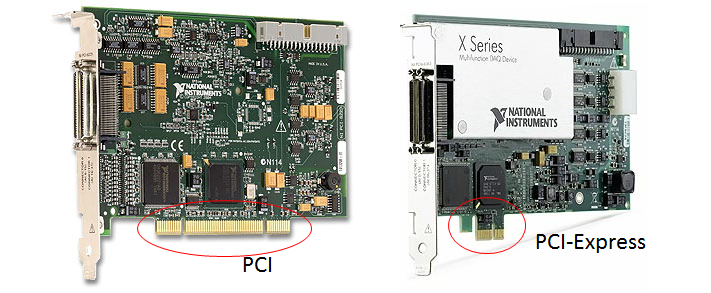
\includegraphics[width=0.8\textwidth]{figuras/pcivspcienational.png}
	\caption{Placas PCI e PCI-Express da National Instruments. \cite{lojanational}}
	\label{figura:pcixpcieni}
\end{figure}

Os modelos de DAQs na forma de extensão de placas para PCs foram bastante comuns na década de 90, porém esta classe de dispositivos podem sofrer interferência eletromagnética e eletrostática devido as máquinas rotativas dos computadores, como os \emph{coolers} e a própria estrutura de barramentos do computador, necessitando de um sistema de proteção contra este tipo de interferência. Atualmente os fabricantes vem disponibilizando sistema de aquisição de dados em uma caixa separada do computador garantindo um isolamento melhor em relação as interferências do computador. O fato de está externo ao computador, permite, também, uma maior mobilidade e menos restrição de espaço podendo ser utilizado em conjunto com \emph{notebooks}, não se limitando apenas a uma máquina, e ainda, em alguns casos, permitindo a comunicação entre DAQs a metros ou quilômetros de distância e o computador. 

Estes dispositivos isolados do computador só foram possíveis porque a comunicação entre o PC e seus periféricos externos evoluiu bastante. Os primeiros dispositivos isolados, ou \emph{stand-alone}, utilizavam principalmente a comunicação serial, RS232 e suas variantes como o RS485, para o caso do meio industrial. Estes padrões ainda são bastante comum no meio industrial e entre dispositivos embarcados, porém, não permite altas taxas de transferência, daí a preferência por placas PCI no passado. Com o surgimento de protocolos de comunicação mais recentes, como a USB, à partir da versão 2.0 e a \emph{Ethernet}, incluindo, mais recentemente, as redes sem fio, os DAQs \emph{stand-alone} com vários canais de alta velocidade, no qual necessita de um tráfego intenso de dados, se tornaram viáveis.

Historicamente os sistemas de aquisição de dados foram criados para atender a necessidade de grandes industrias e centros de pesquisa. Estes tipos de equipamentos, por sua vez, nunca foram baratos, devido a necessidade de equipamentos de alta qualidade, principalmente, devido ao grande poder de compra dos clientes. Por isso, os maiores fabricantes dessa classe de dispositivos possuem soluções com preços pouco convidativos, e quase sempre atrelados a \emph{software} e \emph{hardware} proprietário. Para exemplificar, a \emph{National Instruments} (NI), uma grande fabricante no ramo, vendem DAQs que variam de R\$ 2.087,88 a R\$ 63,540, segundo a loja oficial no Brasil \cite{lojanational}. O uso de \emph{software} e \emph{hardware} proprietários torna comum a prática de venda casada, pois para o funcionamento completo do DAQ é necessário adquirir mais de um produto, um anuncio da DAQ Instruments de um pacote incluindo o DAQ e os softwares necessários para o seu funcionamento exemplifica esta prática. Sozinho o aparelho custa \$59,00, porém, para ter a melhor experiência o fabricante sugere a compra de um pacote de \$244,00 (Figura \ref{figura:vendacasada}).

\begin{figure}
	\centering
	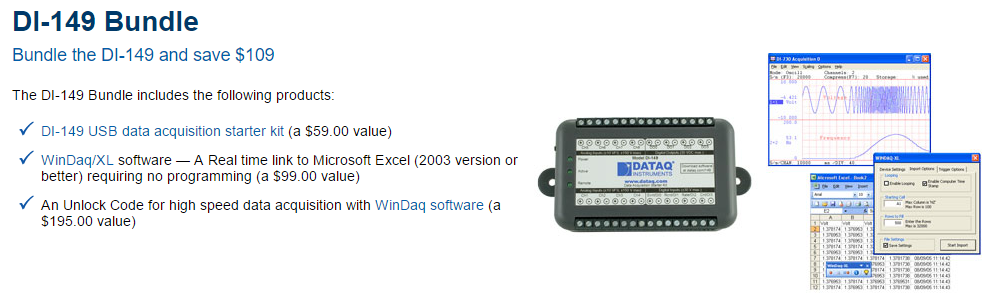
\includegraphics[width=0.9\textwidth]{figuras/bundle.PNG}
	\caption{Exemplo de anúncio de venda casada do Kit DI-149. \cite{dataqcasada}}
	\label{figura:vendacasada}
\end{figure} 

Na topologia padrão de um DAQ conectado a um computador é necessário converter o sinal analógico, geralmente vindo de um sensor, para dados digitais, de tal forma que possa ser reconhecido pelo computador. Esses dados posteriormente serão enviados através de uma interface de comunicação entre o computador e o DAQ. Para que tudo isso seja possível existe uma CPU capaz de gerenciar os dados de entrada conversor analógico digital, ou ADC (\emph{Analog-to-digital converter}), e a interface de comunicação. Um esquemático dessa topologia pode ser visto na figura \ref{figura:esquematico-daq-pc}.

\begin{figure}
	\centering
	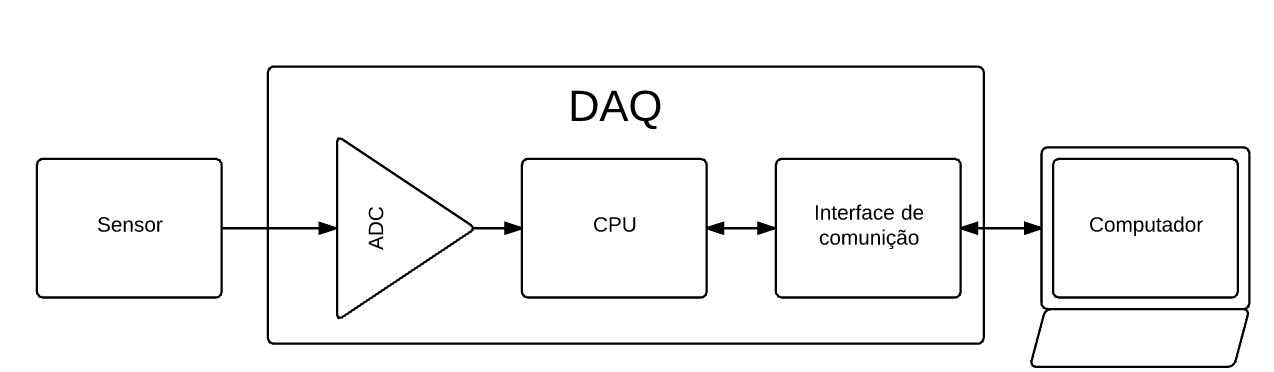
\includegraphics[width=0.9\textwidth]{figuras/daq-esquema.png}
	\caption{Esquemático de um DAQ conectado a um computador (Próprio Autor)}
	\label{figura:esquematico-daq-pc}
\end{figure}

Na verdade, a topologia do DAQ representado na figura \ref{figura:esquematico-daq-pc} é algo bastante comum na eletrônica embarcada, por isso, já vem embutida em alguns microcontroladores. Sistemas embarcados, são dispositivos feitos para um propósitos específico, desde ao controle de um elevador ao gerenciamento de um instrumento de aquisição de dados. Nestes sistemas é comum o uso de microcontroladores, que são computadores dedicados àquela tarefa exclusiva. Muitos microcontroladores, além da CPU e memória, vem com diversos protocolos de comunicação, ADCs, DACs (Digital Analog Converters) embutidos em um único encapsulamento. Essa integração de diversos periféricos em um único \emph{chip} deixa o projeto mais simples e barato, por isso é cada vez mais comum os fabricantes disponibilizarem sistemas cada vez mais completos em um único encapsulamento. Esse conceito é conhecido como \emph{System on Chip}, os famosos SOCs, que estão embarcados nos mais diversos dispositivos, até mesmo em celulares.

Os primeiros microcontroladores surgiram no final do século passado. Inicialmente eles não eram muito acessíveis, tanto na questão de preço quando na complexidade de programação e desenvolvimento. Muito deles tinham que ser programados em \emph{Assembly}, ou linguagem de máquina, por causa da baixa memória disponível. Entretanto, com o tempo os novos modelos vieram com mais memória, mais poder de processamento e periféricos mais avançado, junto a isso, como tudo na tecnologia, surgiu novas ferramentas e compiladores, facilitando bastante o desenvolvimento de dispositivos microcontrolados. Uma grande evolução nesse sentido aconteceu em 2005, quando um grupo de pesquisadores da Itália propuseram uma plataforma de prototipagem de baixo custo, fácil utilização e de código aberto, conhecida como Arduino. O \emph{hardware} do Arduino é uma placa de desenvolvimento completa, ou seja, além do microcontrolador, ela vem com todos os circuitos externos para o seu funcionamento, incluindo fonte de alimentação, regulador de tensão, oscilador externo, entrada USB e pinos de extensão \cite{tedarduino}. Além do \emph{hardware} pronto para o uso o Arduino dispõe uma linguagem de programação que abstrai os elementos de \emph{hardware} do microcontrolador, portanto é possível programar no Arduino sem precisar setar nenhum valor em registradores do microcontrolador, as bibliotecas e funções disponível na linguagem já faz todas as configurações necessárias para o usuário leigo. O fato de ser código aberto e a facilidade de utilização atraiu diversos entusiastas, hobbistas e profissionais para a plataforma, se tornando uma das maiores comunidades, se não a maior, de sistemas embarcados atualmente. 

De uma forma geral, o Arduino, além de aumentar o número de pessoas interessadas em eletrônica, aumentou a quantidade de projetos e velocidade com que eles eram feitos, possibilitando a criação de projetos como tênis que amarra sozinho e impressoras 3D \cite{tenissozinho}. Hoje existem diversos fabricantes que fabricam módulos de expansão para o Arduino conhecidos como Shields. Existem módulos para tudo, controle de motores, relés, conexão \emph{ethernet} e Wi-Fi, \emph{bluetooth}, dentre outros. Com os módulos o usuário só precisa comprar conectores e programar, não havendo a necessidade de criar circuitos complexos na \emph{protoboard} ou fazer placas de circuito impresso.

Depois que o Arduino se tornou popular diversas organizações e empresas resolveram criar suas placas de desenvolvimento \emph{open source}. Na época em que o Arduino foi criado surgiram os primeiros \emph{smartphones}, junto com eles, os SOCs com processadores ARM e GPUs de baixo consumo que permitiu aliar o baixo consumo, dissipação de calor, tamanho portátil e alto desempenho em um único \emph{chip}. Em 2008 a Texas Instruments, uma empresa privada que desenvolve diversos produtos semicondutores como microcontroladores e SOCs com arquitetura ARM para celulares, resolveu criar a Beagleboard em parceria com a Digikey e a Element14, duas empresas do ramo de varejo eletrônico nos EUA. A ideia era demonstrar o poder do SOC  OMAP3530 em uma placa de desenvolvimento do tamanho de cartão de crédito, capaz de rodar uma distribuição Linux portada para ARM incluindo os aplicativos compilado este sistema operacional.  A ideia foi promissora, pois foi uma das pioneiras na área de computadores embarcados, mas o preço de \$125 não fez a placa decolar. O Linux embarcado, ou E-Linux, só se tornou popular quando a fundação Raspberry Pi resolveu criar um produto de mesmo nome por apenas 35 dólares, em fevereiro de 2012. A ideia da fundação era criar uma plataforma de programação de baixíssimo custo \cite{tecmundopi}. Hoje Raspeberry Pi é de longe a \emph{E-Linux board} mais vendida e com a maior comunidade. \emph{E-Linux boards} é o termo utilizado para computadores que rodam linux embarcado.

Junto ao sucesso do Raspberry Pi, surgiram diversas outras opções de empresas e fundações que queria por sua plataforma \emph{open source} com Linux embarcado no mercado, ou atualizá-las como foi o caso da empresa criadora do Beagleboard. Assim aproveitando a onda dos computadores \emph{single board} a Texas Instruments criou o BeagleBone Black. O grande diferencial deste computador em relação ao Raspberry Pi à Beagleboard está nos periféricos. O BBB (Abreviação de Beaglebone Black) tem 65 pinos de extensão, um microcontrolador auxiliar para programação em tempo real, o PRU, e muito mais periféricos que o Raspberry Pi. Para efeito de comparação na tabela \ref{tab:compsingleboardpcs} tem-se o comparitivo entre o Beaglebone Black, Arduino Yun, uma das versões do arduino com Linux embarcado, e o Raspeberry Pi. Pela tabela percebe-se que o BBB é o único concorrente que alia o alto poder de processamento com a grande quantidade de periféricos e I/O, termo inglês para representar os pinos de extensão de entrada, \emph{input}, e saída, \emph{output}. A quantidade elevada de I/Os permitiu a fabricante do Beaglebone criar o conceito de placas de expansão para a \emph{E-Linux board} conhecida como Capes, semelhante aos Shields disponíveis para Arduino. 
	
\begin{table}
	\centering
	\begin{tabular}[c]{c|ccc}
		&Arduino Yun&Beaglebone Black&Raspberry Pi\\ \hline
		CPU&MIPS32&ARM Cortex-A8&ARM1176\\
		CPU Freq.&400Mhz&1Ghz&700Mhz\\ 
		Microcontrolador&ATmega32U4&PRU&Não tem\\ 
		\(\displaystyle \mu \)controlador Freq.&16Mhz&200Mhz&-\\
		RAM&64Mb&512Mb&512Mb\\ 
		GPU&Não tem&PowerVR SGX530&Broadcom VideoCore IV\\ 
		Memória interna&16Mb&4GB&Não tem\\ 
		Memória externa&Micro SD&Micro SD&SD\\ 
		I/O&20&65&17\\
		Ethernet&10/100 Mbit&10/100 Mbit&10/100 Mbit\\ 
		ADC&12x 10bits, 0-5V&7x 12bits 0-1.8V&Não tem\\ 
		PWM&7x&8x&1x\\ 
		UART&2x&4x&1x\\ 
		SPI&1x&2x&2x\\ 
		I2C&1x&2x&1x\\ 
		USB \emph{Host}&1x&1x&2x\\
		USB \emph{Client}&1x&1x&Não tem\\ 
		Video&Não tem&Micro HDMI&HDMI, RCA, DSI\\ 
		Audio&Não tem&Micro HDMI&HDMI, P2\\
		Preço&\$75&\$55&\$35\\ \hline
	\end{tabular}
	\caption{Comparação entre os \emph{E-linux board} \emph{open source} mais usados no mercado \cite{comparisonelinux}.}
	\label{tab:compsingleboardpcs}
\end{table}
	
O Beaglebone Black quando foi lançado fez um relativo sucesso, mais que o seu antecessor, principalmente pela nova política de preço, seu microcontrolador integrado e a quantidade generosa de I/Os e periféricos. Entretanto isso não foi o suficiente para desbancar o Raspberry Pi. Parte disso é devido a forma de como as \emph{E-Linux boards} são utilizadas. A maioria das aplicações desses \emph{single board computers} está na área de computação, como na criação de pequenos servidores, centrais de emulação, \emph{media centers}, câmeras de vigilância, dentre outros. Para isso, as poucas portas e periféricos do Raspberry Pi é o suficiente. Quando há a necessidade de alguma aplicação em tempo real geralmente utiliza-se o Raspberry Pi em conjunto com o Arduino. O outro motivo para o Beaglebone não ter desbancado o Raspberry Pi, foi o fato de este último ter sido lançado muito tarde. Em 2013, quando foi lançado, a comunidade do Pi já estava grande e já existiam outros concorrentes, como a Cubie Board. Além disso, as Capes que poderiam ser um grande diferencial são muito caras e não há muita variedade. Na prática o BBB é uma dos \emph{sigle board computers} mais utilizados, mas está longe de ser a mais popular e o conceito de Capes não engrenou como a fabricante previa.
	
Embora Beaglebone Black tenha todos esses contras, ele ainda é a melhor opção de \emph{E-Linux computer} para a construção de um DAQ. Pois para a criação de um DAQ é necessário um ADC de boa qualidade, uma CPU de alto desempenho para processar todos os dados capturados e interfaces de comunicação de alta velocidade, como Ethernet e USB 2.0. Por isso este trabalho pretende utilizar o Beaglebone Black para criar um sistema de aquisição de dados de baixo custo conectado ao computador pela porta USB. Sistema no qual será utilizado posteriormente para a captura de dados de um acelerômetro analógico industrial, em trabalhos futuros.

	
	\chapter{Fundamentação Teórica}
	\label{ch:theory}
	\section{Componentes do Beaglebone Black}
\label{ch:bbb_components}

No capítulo \ref{ch:introduction} foi introduzido o Beaglebone Black como um mini computador de arquitetura ARM. Esta seção irá mostrar os componentes da placa e os integrados ao SOC Sitara AM335x. Na figura \ref{figura:bbb_components} tem-se uma foto de frente e verso da placa de circuito impresso do BBB, identificando os componentes, e na tabela \ref{tab:bbb_components} identifica a função de cada componente na placa. Para complementar na figura \ref{figura:bbb_soc} mostra os componentes integrados ao SOC Sitara AM3358A, este último disponível na \emph{rev.3} deste produto.

\begin{table}[h]
	\centering
	\begin{tabular}[c]{ccm{10cm}}
		No.&Componente&Função\\ \hline
		1&Sitara AM335x&SOC do BBB contendo diversos componentes integrados incluindo a CPU, GPU e PRU.\\
		2&HDMI Framer&Converte o controlador de LCD do AM335x.\\
		3&Memória RAM&512MB DDR3.\\
		4&eMMC&4GB de memória de armazenamento interna.\\
		5&TPS65217C&Regulador de potência sofisticado com 4 reguladores de tensão LDO controlado por I2C\\
		6&Ethernet PHY&Conecta o processador ARM a conexão física RJ45 com a velocidade de 100Mbit para enviar e 10Mbit para receber.\\
		7&7x LEDs&\emph{Power} LED (azul), 4 \emph{user} LEDs e 2 LEDs (amarelo = dados enviados/ verde = dados recebidos).\\
		8&\emph{Push Buttons}&Liga/Desliga (\emph{Power}), \emph{Reset Button} e \emph{Boot Switch}. Este último seleciona se o deve ser feito \emph{boot} do eMMC ou do cartão micro SD.\\
		9&Micro HDMI&Para conectar em monitores de até 1280x1024@60Hz ou 1920x1080@24Hz.\\
		10&Ethernet RJ45&Conector RJ45.\\
		11&5V DC& \emph{Jack} de 5mm para usar o BBB sem precisar alimentar com o cabo USB.\\
		12&\emph{Slot} micro SD& \emph{Slot} para cartão micro SD;\\
		13&\emph{Serial Debug}&Conector de 6 pinos para acessar o terminal através da conexão serial (UART0).\\
		14&USB 2.0 \emph{Client}&Conector mini-USB 2.0 utilizado para conectar o BBB ao computador.\\
		15&USB 2.0 \emph{Host}&Conector USB-A 2.0 para conectar os periféricos do BBB, como \emph{webcams}, \emph{mouse}, teclado e outros. Pode-se utilizar um \emph{hub} USB para conectar mais de um periférico.\\
		16\&17&Expansões P8 e P9&Soquete de pinos de extensão P8 e P9. Cada soquete tem 2x23 pinos totalizando 92 pinos no total.\\
		18&JTAG&Espaço para conector JTAG, bastante utilizado em testes de placas de circuito impresso. Porém, necessita de \emph{software} e \emph{hardware} adicional.\\
		19&Conector de bateria&É possível soldar estes 4 pinos para adicionar um conector de bateria a placa.\\
		\hline
	\end{tabular}
	\caption{Relação dos componentes do BBB de acordo com a figura \ref{figura:bbb_components} \cite{derekbbb}.}
	\label{tab:bbb_components}
\end{table}

\begin{figure}
	\centering
	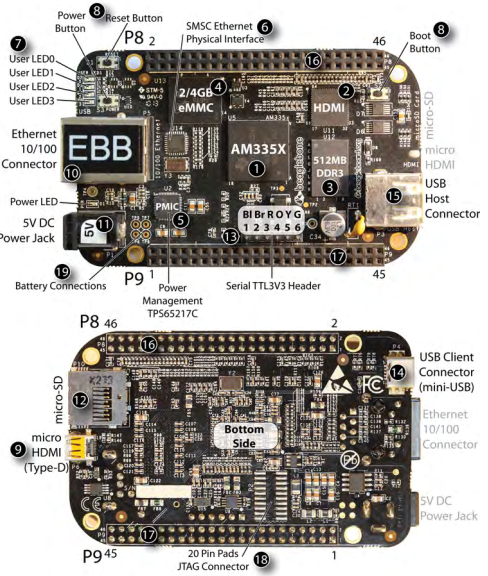
\includegraphics[width=0.6\textwidth]{figuras/bbb_componentes.png}
	\caption{O Beaglebone Black e seus componentes.\cite{derekbbb}}
	\label{figura:bbb_components}
\end{figure}

\begin{figure}
	\centering
	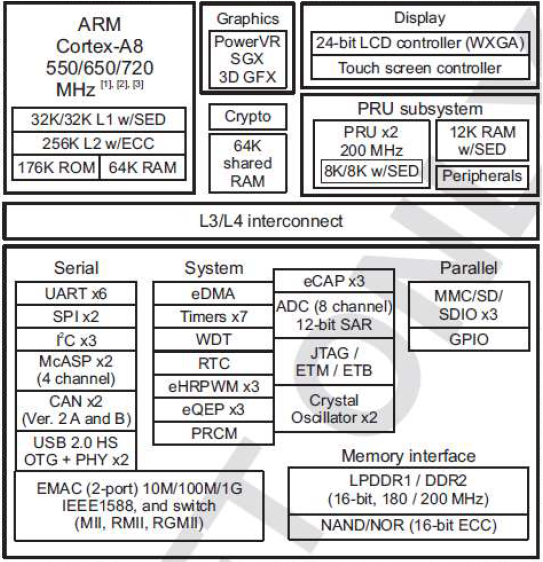
\includegraphics[width=0.6\textwidth]{figuras/bbb_soc.png}
	\caption{Diagrama do Satira AM3358A.\cite{bbbdatasheet}}
	\label{figura:bbb_soc}
\end{figure}

\section{Beaglebone Black e o Linux Embarcado}
\label{ch:bbb_elinux}

Como foi dito nos capítulos anteriores, o Beaglebone Black é um minicomputador completo que é capaz de rodar diversas distribuições de \emph{E-Linux}, Android e outros sistemas operacionais portados para arquitetura ARM. Atualmente a comunidade do Beaglebone portou apenas Android e algumas distribuições Linux, como Debian, Ubuntu, Ångström e Arch Linux. As primeiras versões do Beaglebone Black, mais especificamente as revisões 1 e 2, vinham com Ångström instalado por padrão, uma distribuição linux criada exclusivamente para sistemas embarcados, \emph{tablets}, PDAs, \emph{set top boxes}, roteadores e outros dispositivos baseados na arquitetura ARM \cite{sitebbbang}.

Entretanto, uma parte dos usuários preferiam instalar outra distribuição, como o Ubuntu, pois esta parcela de usuários na maioria das vezes não tinha muita convivência com o Linux e o fato de trabalhar numa distribuição que não tem suas raízes comuns as distrbuições populares para \emph{desktop} tornava o sistema menos amigável. Percebendo a popularidade de tutoriais ensinando como trocar de distribuição, a Texas passou a incluir a distribuição Debian a partir da revisão 3 do Beaglebone Black, lançada em 2014, e revisão mais recente desta placa, além disso, na revisão 3 houve um aumento na memória interna de 2GB para 4GB. Essas adições tornaram o BBB mais atraente para ser usado como computador, pois o espaço extra permitia a instalação de aplicativos para Linux como o \emph{Open Office}, reprodutores de video e editores de imagens.

A nova distribuição facilitou, também, na execução de aplicativos com interface gráfica (GUI) baseados nas \emph{frameworks} GTK+ e Qt, que são bastante populares no Linux \emph{desktop} baseados no Debian e seus derivados, como Ubuntu e Linux Mint. O uso de aplicativos gráficos é bastante comum nas \emph{E-Linux Board} para servir como interface entre o usuário e a máquina. Na figura \ref{figura:bbb_cnc} mostra o exemplo de uma máquina CNC controlada por um Beaglebone e a \emph{cape} K9 CNC I/O. Para controlar a CNC a fabricante da \emph{cape} criou um aplicativo com interface gráfica para Linux onde o usuário é capaz de visualizar o processo e interagir com a CNC.

\begin{figure}[h]
	\centering
	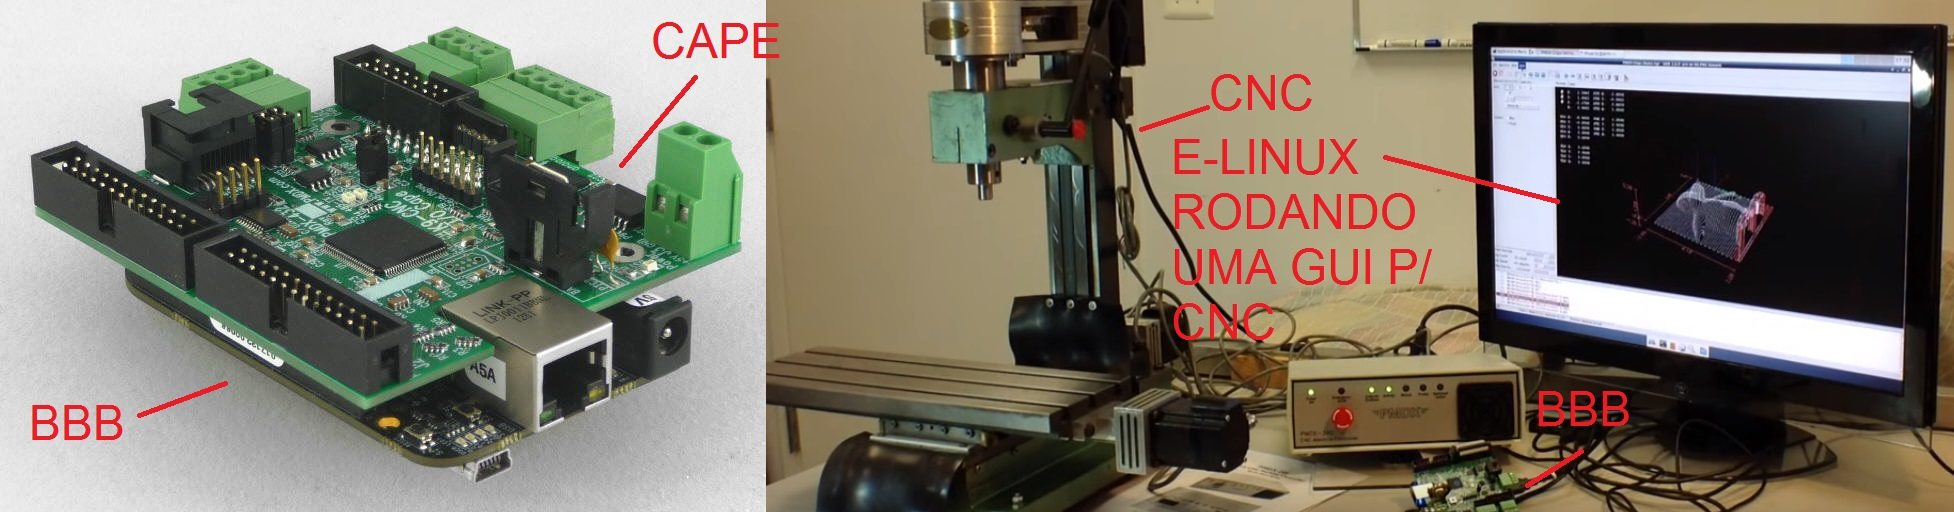
\includegraphics[width=\textwidth]{figuras/cnc_cape.JPG}
	\caption{Beaglebone controlando uma CNC e rodando uma aplicação para CNC simultaneamente.\cite{guicncbbb}}
	\label{figura:bbb_cnc}
\end{figure}

As distribuições baseadas no Debian já vem com as interfaces gráficas e pacotes relacionados instalados por padrão, incluindo aqueles necessários para executar aplicativos criados em Qt ou GTK+. Além disso, essas distribuições vem com diversos outros pacotes que são padrão para a maioria dos usuários Linux, um grande exemplo é o gerenciador de pacotes \emph{apt} que está disponível no Debian, mas não no Ångström.

\subsection{Instalando uma nova distribuição no BBB}

Na seção \ref{ch:bbb_elinux} falo-se da importância de utilizar a distribuição Debian, portanto, se o Beaglebone Black adquirido for anterior a rev.3 deve-se instalar o Debian 7.5 Wheezy, versão de 14/05/2014. Caso o Beaglebone venha uma versão do Debian superior a esta é recomendado fazer o \emph{downgrade} para a versão 7.5, principalmente, se for a versão 8 Jessie ou superior. A versão 7.5 foi projetada pensando, também, nas revisões anteriores a rev. 3, por isso ocupa um pouco menos de 2 Gb, sobrando aproximadamente 2 Gb dos 4Gb da eMMC do BBB, caso este tenha sido adquirido depois de 2014. Esse espaço extra será o suficiente para instalar novos programa, módulos e gerar grandes arquivos de dados. Uma outro motivo fazer o \emph{downgrade} é que neste trabalho e na maioria das bibliografias encontrada na literatura atualmente faz o uso desta versão do Debian, portanto pode haver procedimentos que não sejam os mesmos em versões diferentes, dificultando a reprodução dos experimentos feitos nesta monografia. 

A primeira coisa que deve ser feita para instalar uma nova distribuição é fazer o \emph{download} do sistema operacional, que pode ser baixado na página que contém as  últimas imagens pra Beaglebone Black (\emph{https://beagleboard.org/latest-images}). Caso o leitor desta monografia esteja lendo-a muito tempo depois da sua publicação existe uma alternativa no domínio oficial do Debian (\emph{https://debian.beagleboard.org/images/}), ou ainda, no site do E-Linux (\emph{http://elinux.org/Beagleboard:BeagleBoneBlack\_Debian}). No site das últimas imagens para BBB existem duas versões do Debian 7.5 de 14/05/2014. Uma delas é para utilizar o sistema operacional pelo cartão SD (\emph{without flashing the eMMC}), enquanto a outra grava o sistema operacional na eMMC (\emph{eMMC flasher}). É preferível que o sistema operacional seja instalado na memoria interna do Beaglebone, pois, além desta ter uma taxa de leitura e escrita maior que o cartão SD, ficamos com o \emph{slot} SD livre para ser utilizado em outras ocasiões.

O formato do arquivo baixado é \emph{.img.xz} que é um formato de compactação bastante comum no Linux. Caso o usuário esteja usando o Windows talvez seja necessário fazer o \emph{download} de alguma ferramenta capaz de descompactar este formato de arquivo, visto que alguns aplicativos de descompactação, como WinRar, não trabalham com este tipo de arquivo. Uma sugestão de descompactador capaz de trabalhar com este formato de compactação é o 7-Zip (Disponível em: \emph{http://www.7-zip.org/}), gratuito, \emph{open source} e sem propagandas.

Enquanto a imagem do sistema operacional está sendo baixada, deve-se fazer o \emph{download} de outro programa para gravar a imagem no cartão de memória. Uma sugestão dada pela Wiki do E-Linux é o Win32 Disk Imager (https://sourceforge.net/projects/win32diskimager/) \cite{elinuxupdatebbb}. Quando ambos os arquivos estiverem baixados, descompacte a imagem do Debian que está no formato \emph{.img.xz} e irá obter um arquivo \emph{.img}. Insira o cartão SD no leitor de cartão do seu computador. Abra o Disk Imager selecione a letra correspondente a partição do cartão de memória, selecione a imagem do Debian e clique em gravar como mostra na figura \ref{figura:update_bbb}. Irá aparecer uma caixa de mensagem explicando que esta operação pode danificar os dados no cartão, clique em \emph{yes} espere o processo ser finalizado.

\begin{figure}[h]
	\centering
	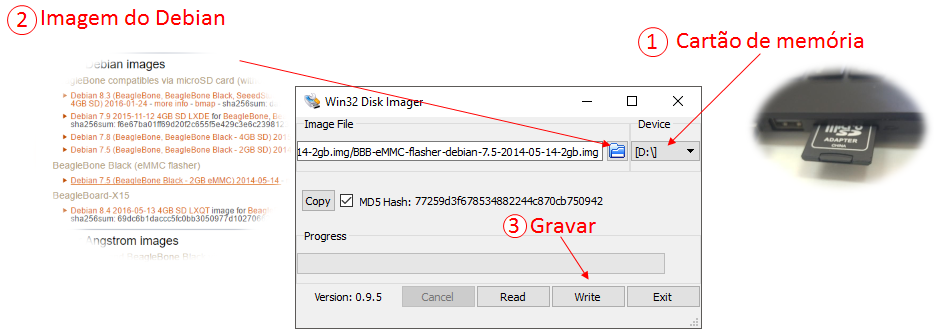
\includegraphics[width=\textwidth]{figuras/update_bbb.png}
	\caption{Gravando a imagem do Debian 7.5 de 14/05/2014 no cartão SD (Próprio Autor)}
	\label{figura:update_bbb}
\end{figure}

Depois do processo de gravação finalizar com sucesso retire o cartão SD do cartão e com o BBB ainda desligado, insira o microSD no \emph{slot} apropriado (Item 12 na figura \ref{figura:bbb_components}). Antes de ligar a placa, mantenha pressionado o \emph{Boot Switch} (Item 8 na figura \ref{figura:bbb_components}), e ainda com o botão pressionado, conecte a porta USB \emph{Client} do Beaglebone (Item 14 na figura \ref{figura:bbb_components}) e ao computador ou alguma fonte de alimentação. Depois dos \emph{User LEDs} (Item 7 na figura \ref{figura:bbb_components}) começarem a piscar solte o \emph{Boot Switch}. A partir daí, o sistema operacional será instalado na eMMC o processo dura cerca de 30 a 40 minutos, durante este tempo não desligue o Beaglebone. Quando a instalação estiver concluída os 4 \emph{User LEDs} irão parar de piscar e ficarão acesos. Neste momento desconecte oo cabo USB da fonte de alimentação retire o cartão SD e conecte novamente o BBB ao computador. Será montada uma partição FAT com o nome \emph{BeagleBone Getting Started} clique nela e abra o arquivo \emph{ID.txt} com o bloco de notas. Se aparecer \emph{BeagleBoard.org BeagleBone Debian Image 2014-04-23
} a atualização da Distro foi realizada com sucesso (Figura \ref{figura:check_bbb_version}).

\begin{figure}[h]
	\centering
	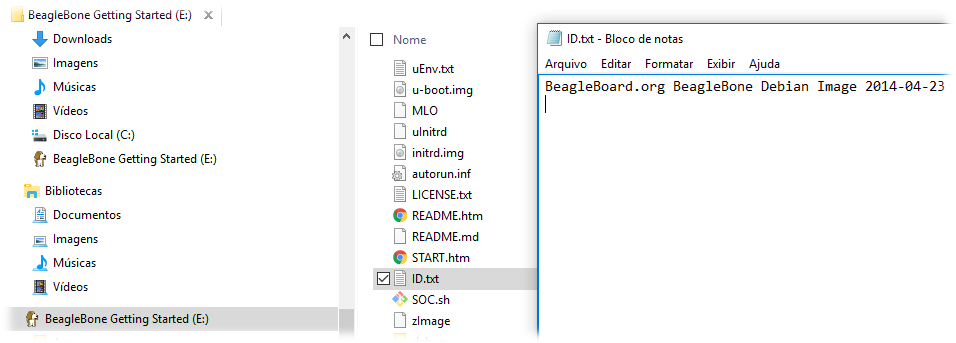
\includegraphics[width=\textwidth]{figuras/check_bbb_version.png}
	\caption{Verificando a atualização do Debian 7.5 foi instalada com sucesso. (Próprio Autor)}
	\label{figura:check_bbb_version}
\end{figure}

\subsection{Comunicando com o BeagleBone Black}

O Beaglebone Black \emph{vanilla}, ou seja, da forma como veio de fábrica, não tem nenhuma interface de interação com o usuário além de alguns \emph{push-bottons} e LEDs indicadores (Itens 7 e 8 da figura \ref{figura:bbb_components}). E isso não é o suficiente para programar ou adicionar alguma nova função a placa de desenvolvimento, a menos que o usuário use o BeagleBone ligado a um monitor, mouse e teclado. Para interagir com o \emph{board computer} sem a necessidade desses aparelhos é necessário se comunicar com o BBB através de um computador hospedeiro. Existem diversas formas de fazer esta comunicação, mas esta seção irá focar na protocolo SSH e no \emph{serial debug}.

$$Vem uma figura aqui$$

O Linux, Mac e sistemas operacionais baseados no Unix, já vem com suporte nativo a SSH através do terminal. Usuários do Windows podem experimentar o \emph{Windows 10 bash shelll}, porém esta solução no momento  , entretanto, usuários do Windows devem baixar um cliente SSH como o PuTTY (Disponível em: \emph{http://www.putty.org/}). Antes de iniciar o processo de comunicação é importante atualizar os \emph{drivers} disponivel em: \emph{http://beagleboard.org/static/beaglebone/latest/README.htm}. Depois da atualização feita e o PuTTY baixado abra este último aplicativo. No campo \emph{Host Name (or IP address)} escreva o IP do BeagleBone que por padrão é $192.168.7.2$. Deixe as outras opções padrões como mostra a figura \ref{}


\subsection{Programando no BeagleBone Black}
\label{ch:bbb_firststeps}

O fato do BeagleBone Black utilizar Linux como sistema operacional o usuário programe em uma infinidade de linguagens de programação, entretanto algumas delas necessitam de passos adicionais. Esta que não vêm instaladas por padrão não serão abordadas nesta seção.

Ao conectar o Beaglebone Black ao computador através da porta USB Client (Item 14 na figura\ref{figura:bbb_components}) será montada a partição FAT \emph{BeagleBone Getting Star


Nas seções anteriores vimos os componentes do BBB e 

Como foi dito na seção \

O fato do BBB já vim com o linux embarcado permite que possa programar em 
	
	
	
	\postextual
		
	\bibliography{biblio}
	
\end{document}